\documentclass[10pt, xcolor=dvipsnames]{beamer} %[handout,red]

\include{math_defs}

\usepackage{graphicx,multimedia,hyperref,xmpmulti}
\usepackage[utf8]{inputenc}
\usepackage[czech]{babel}
\usepackage{bibunits}

\usepackage{verbatim}

% \usepackage[normalem]{ulem}


% transparent objects
\usepackage{transparent}

\newcommand\Warning{%
 \makebox[1.4em][c]{%
 \makebox[0pt][c]{\raisebox{.1em}{\small!}}%
 \makebox[0pt][c]{\color{red}\Large$\bigtriangleup$}}}%
 
\begin{filecontents}{\jobname.bib}
\input{../citace.bib}
\end{filecontents}


\def\Put(#1,#2)#3{\leavevmode\makebox(0,0){\put(#1,#2){#3}}}

% Templating stuff
% \beamertemplatetransparentcovereddynamic
%\colorlet{averagebackgroundcolor}{white}
\setbeamertemplate{itemize items}[circle]
\setbeamertemplate{enumerate items}[square]
\setbeamertemplate{section in toc}[square]
\setbeamercolor*{block title}{fg=white,bg=structure!75!black}
\setbeamercolor*{block body}{bg=structure!10!averagebackgroundcolor}

%\setbeamercolor*{block title example}{fg=white,bg=beamerexample!75!black}
%\setbeamercolor*{block body example}{bg=beamerexample!10!averagebackgroundcolor}
% \usepackage{beamerthemeshadow}
%\setbeamertemplate{background canvas}{\includegraphics [width=0.3\paperwidth]{logo-cxi-cmyk-cz.pdf}}


\setbeamertemplate{footline}{
\includegraphics[width=\paperwidth]{fm_spojovaci.pdf}

\vspace{-2.7mm}

\hspace{5mm}{\bf\inserttitle~ \textcolor{structure}{$\boldsymbol{|}$} \insertdate}

\vspace{-3.5mm}

\hspace{\stretch{1}} \textcolor{white}{\insertframenumber/\inserttotalframenumber} \hspace{2mm}

\vspace{3mm}
}

\definecolor{cxi}{RGB}{193,10,43}
%\definecolor{fm}{RGB}{238,127,0}
%\definecolor{fm}{cmyk}{0.0, 0.563, 1.0, 0.129}
%\definecolor{fm}{HTML}{DE6100}
\definecolor{fm}{RGB}{0,106,179}
\definecolor{mycolor}{HTML}{00CC00}
%\setbeamercolor{structure}{fg=cxi}
\setbeamercolor{structure}{fg=fm}
\setbeamertemplate{frametitle}{\begin{flushleft}\bf\large\insertframetitle\end{flushleft}\par}
\beamertemplateheadempty
\beamertemplatenavigationsymbolsempty
\beamertemplateshadowblocks

\renewcommand{\titlepage}{
{\bf\Large\inserttitle}\\\vspace{3mm}\textit{\insertauthor~ \textcolor{structure}{$\boldsymbol{|}$} \insertdate}

\vspace{1.5cm}
  
\textcolor{structure}{\Large $\boldsymbol{\star}$}~{\bf\large Seminář NTI/iNTEC}
}

% % uncomment if you want outline after each frame
% \AtBeginSection[]
% {
% \frame{\frametitle{Outline}
%   \tableofcontents[currentsection]
% }
% \addtocounter{framenumber}{-1} 
% }

% %%%%%%%%%%%%%%%%%%%%%%%%%%%%%%%%%%%%%%%%%%%%%%%%%%%%%%%%%%%%%%%%%%%%%%%%%%%%%%%%%%%%%%%%%%%%%%%%%%%%%%%%%5
% % ***************************************** SYMBOLS
% \def\div{{\rm div}}
% \def\Lapl{\Delta}
% \def\grad{\nabla}
% \def\supp{{\rm supp}}
% \def\dist{{\rm dist}}
% %\def\chset{\mathbbm{1}}
% \def\chset{1}
% 
% \def\Tr{{\rm Tr}}
% \def\sgn{{\rm sgn}}
% \def\to{\rightarrow}
% \def\weakto{\rightharpoonup}
% \def\imbed{\hookrightarrow}
% \def\cimbed{\subset\subset}
% \def\range{{\mathcal R}}
% \def\leprox{\lesssim}
% \def\argdot{{\hspace{0.18em}\cdot\hspace{0.18em}}}
% \def\Distr{{\mathcal D}}
% \def\calK{{\mathcal K}}
% \def\FromTo{|\rightarrow}
% \def\convol{\star}
% \def\impl{\Rightarrow}
% \DeclareMathOperator*{\esslim}{esslim}
% \DeclareMathOperator*{\esssup}{ess\,sup}
% \DeclareMathOperator{\ess}{ess}
% \DeclareMathOperator{\osc}{osc}
% \DeclareMathOperator{\curl}{curl}
% 
% %\def\Ess{{\rm ess}}
% %\def\Exp{{\rm exp}}
% %\def\Implies{\Longrightarrow}
% %\def\Equiv{\Longleftrightarrow}
% % ****************************************** GENERAL MATH NOTATION
% \def\Real{{\rm\bf R}}
% \def\Rd{{{\rm\bf R}^{\rm 3}}}
% \def\RN{{{\rm\bf R}^N}}
% \def\D{{\mathbb D}}
% \def\Nnum{{\mathbb N}}
% \def\Measures{{\mathcal M}}
% \def\d{\,{\rm d}}               % differential
% \def\sdodt{\genfrac{}{}{}{1}{\rm d}{{\rm d}t}}
% \def\dodt{\genfrac{}{}{}{}{\rm d}{{\rm d}t}}
% 
% \def\vc#1{\mathbf{\boldsymbol{#1}}}     % vector
% \def\tn#1{{\mathbb{#1}}}    % tensor
% \def\abs#1{\lvert#1\rvert}
% \def\Abs#1{\bigl\lvert#1\bigr\rvert}
% \def\bigabs#1{\bigl\lvert#1\bigr\rvert}
% \def\Bigabs#1{\Big\lvert#1\Big\rvert}
% \def\ABS#1{\left\lvert#1\right\rvert}
% \def\norm#1{\bigl\Vert#1\bigr\Vert} %norm
% \def\close#1{\overline{#1}}
% \def\inter#1{#1^\circ}
% \def\ol#1{\overline{#1}}
% \def\ul#1{\underline{#1}}
% \def\eqdef{\mathrel{\mathop:}=}     % defining equivalence
% \def\where{\,|\,}                    % "where" separator in set's defs
% \def\timeD#1{\dot{\overline{{#1}}}}
% \def\avg#1{\langle{#1}\rangle}     % average
% 
% % ******************************************* USEFULL MACROS
% \def\RomanEnum{\renewcommand{\labelenumi}{\rm (\roman{enumi})}}   % enumerate by roman numbers
% \def\rf#1{(\ref{#1})}                                             % ref. shortcut
% \def\prtl{\partial}                                        % partial deriv.
% \def\Names#1{{\scshape #1}}
% \def\rem#1{{\parskip=0cm\par!! {\sl\small #1} !!}}
% 
% \def\Xint#1{\mathchoice
% {\XXint\displaystyle\textstyle{#1}}%
% {\XXint\textstyle\scriptstyle{#1}}%
% {\XXint\scriptstyle\scriptscriptstyle{#1}}%
% {\XXint\scriptscriptstyle\scriptscriptstyle{#1}}%
% \!\int}
% \def\XXint#1#2#3{{\setbox0=\hbox{$#1{#2#3}{\int}$}
% \vcenter{\hbox{$#2#3$}}\kern-.5\wd0}}
% \def\ddashint{\Xint=}
% \def\dashint{\Xint-}
% 
% % ******************************************* DOCUMENT NOTATIONS
% % document specific
% \def\rh{\varrho}
% \def\vl{{\vc{u}}}
% \def\th{\vartheta}
% \def\vx{\vc{x}}
% \def\vX{\vc{X}}
% \def\vr{\vc{r}}
% \def\veta{\vc{\eta}}
% \def\dx{\,\d\vx}
% \def\dt{\,\d t}
% \def\bulk{\zeta}
% \def\cS{\close{S}}
% \def\eps{\varepsilon}
% \def\phi{\varphi}
% \def\Bog{{\mathcal B}}
% \def\Riesz{{\mathcal R}}
% \def\distr{\mathcal D}
% \def\Item{$\bullet$}
% 
% \def\MEtst{\mathcal T}
%***************************************************************************
\setbeamercolor{my blue}{fg=blue}
\def\blue#1{{\usebeamercolor[fg]{my blue} #1}}

%%%%%%%%%%%%%%%%%%%%%%%%%%%%%%%%%%%%%%%%%%%%%%%%%%%%%%%%%%%%%%%%%%%%%%%%%%%%%%%%%%%%%%%%%%%%%%%%%%%%%%%%%%
%MY:

%TABLE
\usepackage{colortbl} %colored table
\usepackage{hhline} %double hlines
\usepackage{array}
\usepackage{booktabs}
\usepackage{subfig}

\newcommand{\figpath}{../graphics/}
\newcommand{\oldresults}{old_results/}
\newcommand{\results}{th_results/}
% \usepackage{amsmath, amsthm, amssymb}
% \usepackage{mathtools}
% \usepackage{esint}

%DATES:
\newcommand{\dst}{\textsuperscript{st}}
\newcommand{\dnd}{\textsuperscript{nd}}
\newcommand{\drd}{\textsuperscript{rd}}
\newcommand{\dth}{\textsuperscript{th}}

%COLORFUL UNDERLINE
\newcommand{\rul}[2]{\textcolor{#1}{\underline{\textcolor{black}{#2}}}}

%FONT SIZES available:
%     \tiny
%     \scriptsize
%     \footnotesize
%     \small
%     \normalsize
%     \large
%     \Large
%     \LARGE
%     \huge
%     \Huge 

%%%%%%%%%%%%%%%%%%%%%%%%%%%%%%%%%%%%%%%%%%%%%%%%%%%%%%%%%%%%%%%%%%%%%%%%%%%%%%%%%%%%%%%%%%%%%%%%%%%%%%%%%5

% SETTING TITLE PAGE MEMBERS
\title{Seznámení s verzovacím systémem Git\\
      \textcolor{lightgray}{v souvislosti s Flow123d, Geompop, bgem}}
\author{{\bf Pavel Exner}}
\institute{TECHNICAL UNIVERSITY OF LIBEREC}
\date{29 leden 2019}


\begin{document}


% { %%%%%%%%%%%%%%%%%%%%%%%%%%%%%%%%%%%%%%%%%%%%%%%   CZECH TITLEPAGE   %%%%%%%%%%%%%%%%%%%%%%%%%%%%%%%%%%%%%%%%%%%%%%%%%%%
%   \setbeamertemplate{background canvas}{\includegraphics [width=0.5\paperwidth]{logos/logo-cxi-cmyk-cz.pdf}}
%   \setbeamertemplate{footline}{\includegraphics[width=\paperwidth]{logos/cxi-spojovaci.png}
% 
%     \vspace{-6mm}
% 
%     \hspace{9mm}
%     %{\bf TECHNICKÁ UNIVERZITA V LIBERCI \textcolor{structure}{$\boldsymbol{|}$ Ústav pro nanomateriály, pokročilé technologie a inovace}}
%     Studentská 1402/2 \textcolor{structure}{$\boldsymbol{|}$} 461 17 Liberec 1 \textcolor{structure}{$\boldsymbol{|}$} www.cxi.tul.cz
% 
%     \vspace{-3.1mm}
% 
%     \hspace{\stretch{1}} \textcolor{white}{\insertframenumber/\inserttotalframenumber} \hspace{2mm}
% 
%     \vspace{3mm}
%     }
%   \frame{
% 	\vspace{1cm}
% 	\titlepage
%   }
% } %%%%%%%%%%%%%%%%%%%%%%%%%%%%%%%%%%%%%%%%%%%%   END CZECH TITLEPAGE   %%%%%%%%%%%%%%%%%%%%%%%%%%%%%%%%%%%%%%%%%%%%%%%%%%%
% 
{ %%%%%%%%%%%%%%%%%%%%%%%%%%%%%%%%%%%%%%%%%%%%%%   ENGLISH TITLEPAGE   %%%%%%%%%%%%%%%%%%%%%%%%%%%%%%%%%%%%%%%%%%%%%%%%%%%
  \setbeamertemplate{background canvas}
  {
    \hspace{5mm}
    
\includegraphics [width=0.5\paperwidth]{logo-fm-cmyk-en.pdf}
  }
%   {
%   \hspace{20pt}
%     \vspace{15pt}
%     
%     \includegraphics [width=0.3\paperwidth]{logo-flow-123d-color.pdf} \hspace{40pt}
%     
\includegraphics [width=0.4\paperwidth]{../logos/logo-fm-cmyk-en.pdf}
%     \hspace{5mm}
%     
\includegraphics [width=0.5\paperwidth]{../logos/logo-fm-cmyk-en.pdf}
%   }
  \setbeamertemplate{footline}{
\includegraphics[width=\paperwidth]{fm_spojovaci.pdf}

%     \vspace{-2.3mm}
    \vspace{-2.3mm}

    \hspace{9mm}
    %{\bf TECHNICAL UNIVERSITY OF LIBEREC \textcolor{structure}{$\boldsymbol{|}$ Institue for Nanomaterials, Advanced Technologies and Innovation}}
    %Studentská 1402/2 \textcolor{structure}{$\boldsymbol{|}$} 461 17 Liberec 1 \textcolor{structure}{$\boldsymbol{|}$} www.cxi.tul.cz
    Studentská 1402/2 \textcolor{structure}{$\boldsymbol{|}$} 461 17 Liberec 1 \textcolor{structure}{$\boldsymbol{|}$} www.fm.tul.cz

    \vspace{-3.5mm}

    \hspace{\stretch{1}} \textcolor{white}{\insertframenumber/\inserttotalframenumber} \hspace{2mm}

    \vspace{3mm}
    }
  \frame{
    \vspace{1cm}
    \titlepage
  }
} %%%%%%%%%%%%%%%%%%%%%%%%%%%%%%%%%%%%%%%%%%%%%%  END ENGLISH TITLEPAGE   %%%%%%%%%%%%%%%%%%%%%%%%%%%%%%%%%%%%%%%%%%%%%%%%%%%


% \begin{frame}
%   \begin{figure}
%         \vspace{-5pt}
%         \begin{center}   
%           \hspace{-10pt}
%           \includegraphics[width=1.05\textwidth]{\figpath liberec/mapa_lbc.pdf}
%         \end{center}
%   \end{figure}
%   
%   \begin{overlayarea}{\linewidth}{\textwidth}
%   \onslide<1>
%     {
%         \vspace{-6.5cm}
%         \hspace{5.6cm}\includegraphics[width=0.29\textwidth]{\figpath liberec/13-Jested.jpg}  
%         
%         \vspace{-4.3cm}
%         \hspace{7cm} \includegraphics[width=0.14\textwidth]{TUL_logo.pdf}
%     }
%     
%   \end{overlayarea}
% \end{frame}

\begin{frame}
  \frametitle{Proč používat verzovací systém?}
  
  \begin{itemize}
    \setlength\itemsep{10pt}
    \item spolupracuji v týmu a chci umět kombinovat změny na jednom souboru od více uživatelů
    \item chci mít zálohu
    \item chci mít přístup k historii změn\\ (návrat k funkčnímu stavu, slepé uličky)
    \item chci mít zdokumentovanou historii změn
    \item chci se podílet na open-source projektech
  \end{itemize}
  
  \vspace{0.5cm}
  \fbox{\parbox{\textwidth}{\centering Především textové soubory!}}
  
\end{frame}


\begin{frame}
  \frametitle{A proč i já, uživatel?}
  
  \vspace{10pt}
  \begin{itemize}
    \setlength\itemsep{10pt}
    \item chci zálohovat/sdílet svůj kód
    \item chci, aby ostatní mohli vylepšit můj kód
    \item chci pomoct ostatním vylepšit jejich kód
    \item nechci dokola vynalézat kolo
    \item píšu/píšeme publikaci
  \end{itemize}
\end{frame}

\begin{frame}
  \frametitle{Git a Github}
  
  \Put(200,20){
\includegraphics[width=0.25\textwidth]{Git-Logo-2Color.eps}}
  \begin{itemize} \setlength\itemsep{10pt}
    \item distribuovaný systém správy verzí
    \item free \& open source
    \item nelineární vývoj -- snadné vytváření a slučování větví
    \item přístup přes protokoly http, ftp, ssh
    \item podpora jiných systémů (cvs, svn)
    \item bohaté webové rozhraní Github
  \end{itemize}
  
  \vspace{0.5cm}
  \begin{itemize} \setlength\itemsep{10pt}
    \item práva k repozitáři -- owner / contributor / others
    \item fork - kopie repozitáře do vlastního repozitáře
  \end{itemize}

\end{frame}

\begin{frame}
  \frametitle{Princip verzování změn I}
  
  \vspace{10pt}
  \centering
  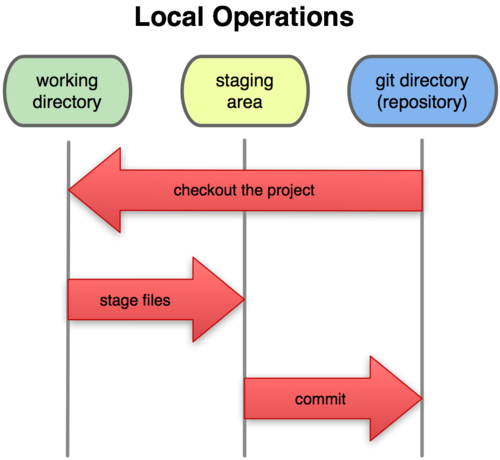
\includegraphics[width=0.75\textwidth]{staging_index.png}

\end{frame}
\begin{frame}
  \frametitle{Princip verzování změn II}
  
  \vspace{10pt}
  \centering
  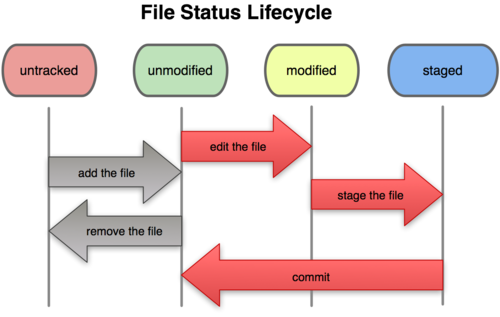
\includegraphics[width=0.75\textwidth]{file_lifecycle.png}

\end{frame}


\begin{frame}[fragile]
  \frametitle{\texttt{https} vs \texttt{ssh} access}
  
  \Put(200,100){
\includegraphics[width=0.25\textwidth]{Git-Logo-2Color.eps}}
  \begin{itemize}
    \setlength\itemsep{10pt}
    \item https připojení (každá akce ve směru local$\rightarrow$remote vyžaduje přihlášení)
    \item SSH generování klíče (Linux shell, Git bash):\\
        \begin{enumerate} \setlength\itemsep{6pt}
          \item \verb'ssh-keygen -t rsa -b 4096 -C "pavel.exner@tul.cz"'{\color{gray}\verb' -f my_rsa'}
          \item vygenerováno: \verb'id_rsa' a \verb'id_rsa.pub' v adr. \verb'~/.ssh/'
          \item zkopírovat veřejný klíč -- obsah \verb'id_rsa.pub' -- do:\\ Github $\rightarrow$ Settings $\rightarrow$ SSH and GPG keys $\rightarrow$ New SSH key
        \end{enumerate}
  \end{itemize}

\end{frame}

\begin{frame}[fragile]
  \frametitle{Git commands I}
  
  \verb'git clone https://github.com/Paulie14/git-seminar.git'\\
  {\color{gray} \verb'git clone git@github.com:Paulie14/git-seminar.git ./my_repos' }
  
  \verb'git checkout master' \hfill\textcolor{gray}{přepni se do hlavní větve}\\
  \verb'git pull' \hfill\textcolor{gray}{stáhni aktuální stav vzdáleného repozitáře}\\
  \verb'git checkout -b PE_new_feature' \hfill\textcolor{gray}{odděl svoji vývojou větev}\\
  
  \vspace{0.5cm}
  \textcolor{gray}{$\ldots$}\\
  \textcolor{gray}{\emph{kóduju o sto šest}}\\
  \textcolor{gray}{$\ldots$}\\
\end{frame}

\begin{frame}[fragile]
  \frametitle{Git commands II}
  
  \textcolor{gray}{$\ldots$}\\
  \verb'git status' \hfill\textcolor{gray}{ukaž, které soubory se změnily}\\
  \verb'git diff' \hfill\textcolor{gray}{ukaž konkrétní změny v souborech}\\
  \verb'git add my_briliant_script.py' \hfill\textcolor{gray}{přidej provedenou změnu}\\
  \verb'git status' \hfill\textcolor{gray}{zkontroluj změny ve stage}\\
  \verb'git commit -m "Popis zmeny."' \hfill\textcolor{gray}{proveď změnu a přidej popis}\\
  \textcolor{gray}{$\ldots$}
  
  \vspace{0.5cm}
  {\color{red}\rule{\textwidth}{1pt}}
  \verb'git push origin PE_new_feature'\\ \hfill\textcolor{gray}{pošli změny do vzdáleného repozitáře}\\
  \textcolor{gray}{$\ldots$}
\end{frame}

\begin{frame}[fragile]
  \frametitle{Git commands III}
  
  \textcolor{gray}{$\ldots$}\\
  \verb'git checkout master' \hfill\textcolor{gray}{přepni se do hlavní větve}\\
  \verb'git pull' \hfill\textcolor{gray}{stáhni aktuální stav vzdáleného repozitáře}\\
  \verb'git checkout PE_new_feature' \hfill\textcolor{gray}{přepni do své vývojové větve}\\
  
  \vspace{0.5cm}
  \verb'git merge master' \hfill\textcolor{gray}{proveď merge z master větve}\\
  \textcolor{gray}{$\ldots$}\textcolor{gray}{vyřeš konflikty}\textcolor{gray}{$\ldots$}\\
  {\color{gray} \verb'git stage'}\\
  {\color{gray} \verb'git commit'}
  
  \vspace{0.5cm}
  {\color{red}\rule{\textwidth}{1pt}}
  \verb'git push origin PE_new_feature'\\ \hfill\textcolor{gray}{pošli merge do vzdáleného repozitáře}\\
  \textcolor{gray}{Vytvoř Pull request}
\end{frame}


\begin{frame}[fragile]
  \frametitle{Git commands IV}
  
  Diff tool: např. Kdiff3 (\url{http://kdiff3.sourceforge.net/})
  
  \vspace{0.5cm}
  Nastavení nástroje pro \verb'merge':
  
  \vspace{0.5cm}
  \verb'git config --global --add merge.tool kdiff3'\\
  \verb'git config --global --add mergetool.kdiff3.path'\\
      \hfill\verb"C:/Program Files/KDiff3/kdiff3.exe"'\\
  
  \vspace{0.5cm}
  \verb'git config --global --add diff.guitool kdiff3'\\
  \verb'git config --global --add difftool.kdiff3.path'\\
      \hfill\verb"C:/Program Files/KDiff3/kdiff3.exe"'

\end{frame}



\begin{frame}[fragile]
  \frametitle{Git Cola}
  
  \Put(200,0){
\includegraphics[width=0.25\textwidth]{Git-Cola.png}}
  \begin{itemize}
    \item \url{https://git-cola.github.io/}
    \item GUI for Git
  \end{itemize}
  
  \vspace{1cm}
  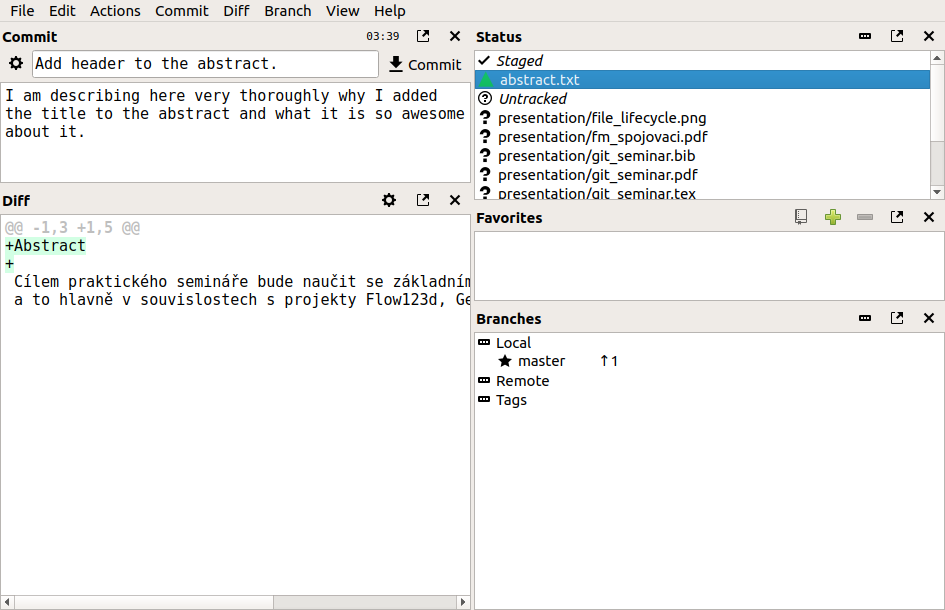
\includegraphics[width=0.48\textwidth]{git-cola-screen.png}
  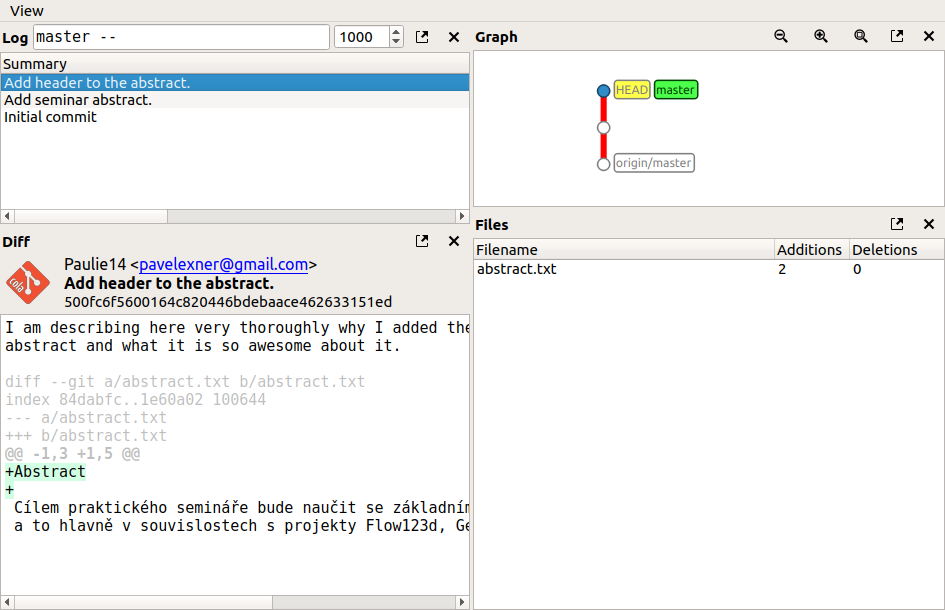
\includegraphics[width=0.48\textwidth]{git-cola-DAG-screen.png}
\end{frame}


\begin{frame}
  \frametitle{Repozitáře}

  \begin{itemize}
    \setlength\itemsep{15pt}
    \item \url{https://github.com/flow123d/flow123d}
    \item \url{https://github.com/GeoMop/GeoMop}
    \item \url{https://github.com/GeoMop/bgem}
  \end{itemize}

\end{frame}

\begin{frame}[fragile]
  \frametitle{Issues a šablony}

  \begin{itemize}
    \setlength\itemsep{15pt}
    \item v repozitářích vytvořeny šablony pro Issue (\verb'.github/ISSUE_TEMPLATES/*.md')
    \item automaticky přiřadí \verb'Assignee', \verb'Label', $\ldots$
    \item obsahuje defaultní název a strukturu Issue
  \end{itemize}

  \begin{center}
  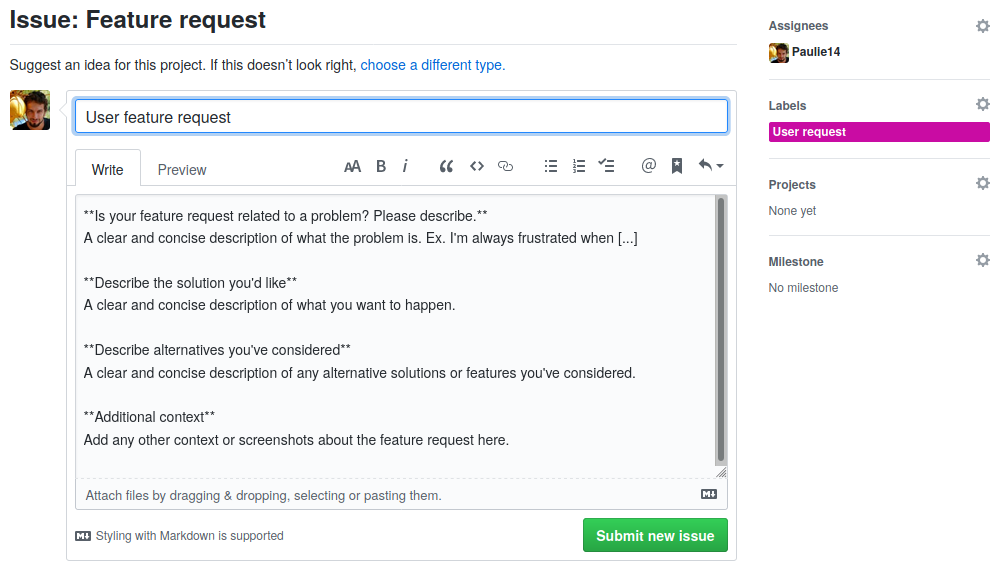
\includegraphics[width=0.65\textwidth]{issue_template.png}
  \end{center}
\end{frame}

\begin{frame}[fragile]
  \frametitle{Your turn!}

  \begin{itemize}\setlength\itemsep{10pt}
    \item proveďte Fork repozitáře \verb'bgem'
    \item naklonujte si svůj nový Fork
    \item oddělte si větev
    \item proveďte změny
    \item odešlete změny v nové větvi na Remote
  \end{itemize}
  
  {\color{green}\rule{\textwidth}{1pt}}
  \begin{itemize}\setlength\itemsep{10pt}
    \item otevřete si repozitář v Pycharmu a zprovozněte
  \end{itemize}
\end{frame}


\begin{frame}[fragile]
  \frametitle{Pro pokročilé}

  \begin{itemize}
    \setlength\itemsep{15pt}
    \item slučování větví
    \item pull request
    \item pull request z Forku do původního repozitáře
    \item submoduly (repozitář součástí repozitáře)
  \end{itemize}
\end{frame}

\end{document}
